% Options for packages loaded elsewhere
\PassOptionsToPackage{unicode}{hyperref}
\PassOptionsToPackage{hyphens}{url}
\documentclass[
  ignorenonframetext,
]{beamer}
\newif\ifbibliography
\usepackage{pgfpages}
\setbeamertemplate{caption}[numbered]
\setbeamertemplate{caption label separator}{: }
\setbeamercolor{caption name}{fg=normal text.fg}
\beamertemplatenavigationsymbolsempty
% remove section numbering
\setbeamertemplate{part page}{
  \centering
  \begin{beamercolorbox}[sep=16pt,center]{part title}
    \usebeamerfont{part title}\insertpart\par
  \end{beamercolorbox}
}
\setbeamertemplate{section page}{
  \centering
  \begin{beamercolorbox}[sep=12pt,center]{section title}
    \usebeamerfont{section title}\insertsection\par
  \end{beamercolorbox}
}
\setbeamertemplate{subsection page}{
  \centering
  \begin{beamercolorbox}[sep=8pt,center]{subsection title}
    \usebeamerfont{subsection title}\insertsubsection\par
  \end{beamercolorbox}
}
% Prevent slide breaks in the middle of a paragraph
\widowpenalties 1 10000
\raggedbottom
\AtBeginPart{
  \frame{\partpage}
}
\AtBeginSection{
  \ifbibliography
  \else
    \frame{\sectionpage}
  \fi
}
\AtBeginSubsection{
  \frame{\subsectionpage}
}
\usepackage{iftex}
\ifPDFTeX
  \usepackage[T1]{fontenc}
  \usepackage[utf8]{inputenc}
  \usepackage{textcomp} % provide euro and other symbols
\else % if luatex or xetex
  \usepackage{unicode-math} % this also loads fontspec
  \defaultfontfeatures{Scale=MatchLowercase}
  \defaultfontfeatures[\rmfamily]{Ligatures=TeX,Scale=1}
\fi
\usepackage{lmodern}
\ifPDFTeX\else
  % xetex/luatex font selection
\fi
% Use upquote if available, for straight quotes in verbatim environments
\IfFileExists{upquote.sty}{\usepackage{upquote}}{}
\IfFileExists{microtype.sty}{% use microtype if available
  \usepackage[]{microtype}
  \UseMicrotypeSet[protrusion]{basicmath} % disable protrusion for tt fonts
}{}
\makeatletter
\@ifundefined{KOMAClassName}{% if non-KOMA class
  \IfFileExists{parskip.sty}{%
    \usepackage{parskip}
  }{% else
    \setlength{\parindent}{0pt}
    \setlength{\parskip}{6pt plus 2pt minus 1pt}}
}{% if KOMA class
  \KOMAoptions{parskip=half}}
\makeatother
\usepackage{longtable,booktabs,array}
\newcounter{none} % for unnumbered tables
\usepackage{calc} % for calculating minipage widths
\usepackage{caption}
% Make caption package work with longtable
\makeatletter
\def\fnum@table{\tablename~\thetable}
\makeatother
\usepackage{graphicx}
\makeatletter
\newsavebox\pandoc@box
\newcommand*\pandocbounded[1]{% scales image to fit in text height/width
  \sbox\pandoc@box{#1}%
  \Gscale@div\@tempa{\textheight}{\dimexpr\ht\pandoc@box+\dp\pandoc@box\relax}%
  \Gscale@div\@tempb{\linewidth}{\wd\pandoc@box}%
  \ifdim\@tempb\p@<\@tempa\p@\let\@tempa\@tempb\fi% select the smaller of both
  \ifdim\@tempa\p@<\p@\scalebox{\@tempa}{\usebox\pandoc@box}%
  \else\usebox{\pandoc@box}%
  \fi%
}
% Set default figure placement to htbp
\def\fps@figure{htbp}
\makeatother
\setlength{\emergencystretch}{3em} % prevent overfull lines
\providecommand{\tightlist}{%
  \setlength{\itemsep}{0pt}\setlength{\parskip}{0pt}}
% Auto-generated by infrastructure/rendering/_pdf_latex_helpers.py::extract_math_font_preamble.
% Minimal header passed to Pandoc via -H so Beamer slides pick up the same math font
% as the combined-PDF path. Adjust the manuscript's preamble.md to change the font globally.
\usepackage{unicode-math}
\setmathfont{latinmodern-math.otf}

% Slide layout defaults for warning-clean scientific decks.
\usepackage{etoolbox}
\IfFileExists{xurl.sty}{\usepackage{xurl}}{}
\IfFileExists{seqsplit.sty}{\usepackage{seqsplit}}{\newcommand{\seqsplit}[1]{#1}}
\protected\def\breakseq#1{\seqsplit{#1}}
\protected\def\breaktt#1{\begingroup\ttfamily\seqsplit{#1}\endgroup}
\setlength{\emergencystretch}{6em}
\tolerance=5000
\hbadness=10000
\hfuzz=1pt
\setlength{\tabcolsep}{2pt}
\AtBeginEnvironment{longtable}{\tiny\renewcommand{\arraystretch}{0.86}\setlength{\tabcolsep}{1pt}}
\AtBeginEnvironment{tabular}{\tiny\renewcommand{\arraystretch}{0.86}\setlength{\tabcolsep}{1pt}}

% Natbib and cross-reference fallbacks — slides don't load natbib
% or cleveref, but combined-PDF manuscript prose may emit these
% commands. The fallback renders citations as a bracketed key list
% and cross-references as detokenized labels so slides don't fail on
% undefined control sequences or raw underscores. \providecommand is
% a no-op if packages load later.
\providecommand{\citep}[1]{[#1]}
\providecommand{\citet}[1]{#1}
\providecommand{\citealp}[1]{#1}
\providecommand{\citeauthor}[1]{#1}
\providecommand{\citeyear}[1]{#1}
\providecommand{\cref}[1]{\texttt{\detokenize{#1}}}
\providecommand{\Cref}[1]{\texttt{\detokenize{#1}}}
\usepackage{bookmark}
\IfFileExists{xurl.sty}{\usepackage{xurl}}{} % add URL line breaks if available
\urlstyle{same}
% fallback for those not using the hyperref driver hyperxmp:
\makeatletter
\@ifundefined{xmpquote}{\newcommand{\xmpquote}[1]{#1}}{}
\makeatother
\hypersetup{
  hidelinks,
  pdfcreator={LaTeX via pandoc}}

\author{\texorpdfstring{}{}}
\date{}

\begin{document}

\section{Evaluation: Gate Criteria, QA Probes, and Failure
Discovery}\label{evaluation-gate-criteria-qa-probes-and-failure-discovery}

\begin{frame}[allowframebreaks]{Evaluation: Gate Criteria, QA Probes,
and Failure Discovery}
The evaluation section is configured to name readiness criteria, connect
criteria to artifacts, separate local checks from publication readiness,
and make failure probes visible. The local readiness surface is not a
human preference score; it is a set of deterministic checks that connect
generated manuscript claims to source files and pipeline gates.

The active criteria use analysis, copy, pytest, validation as gate
labels and inspect artifacts such as token-injection flow, quality-gate
matrix, configured-field figures. A passing run means the exemplar is
locally render-ready: placeholders resolve, token provenance is present,
figure references are registered, evidence scanning has not found
unsupported numbers, and project design overlays remain internally
consistent.

That readiness is deliberately narrower than publication readiness. A
local pass does not imply a standalone DOI, external release, reader
preference result, or empirical validation. It means the tracked project
tree can regenerate the committed artifact surface through its declared
pipeline.

The QA probes are Method row completeness, Field-origin visibility,
Placeholder survival, Provenance completeness, Section-switch
observability, Figure registry coverage, Method-figure alignment,
Evidence cleanliness, Fork readiness, Copied-output parity, Digest
invariant review, Claim-ledger alignment, Review packet completeness,
Fork migration sufficiency. They are phrased as questions so they can be
reused by reviewers and by forks of the exemplar: did the placeholder
disappear, did the provenance survive, did the figure registry cover
every reference, and did copied outputs preserve the same evidence
surface that validation inspected?

\begin{figure}
\centering
\pandocbounded{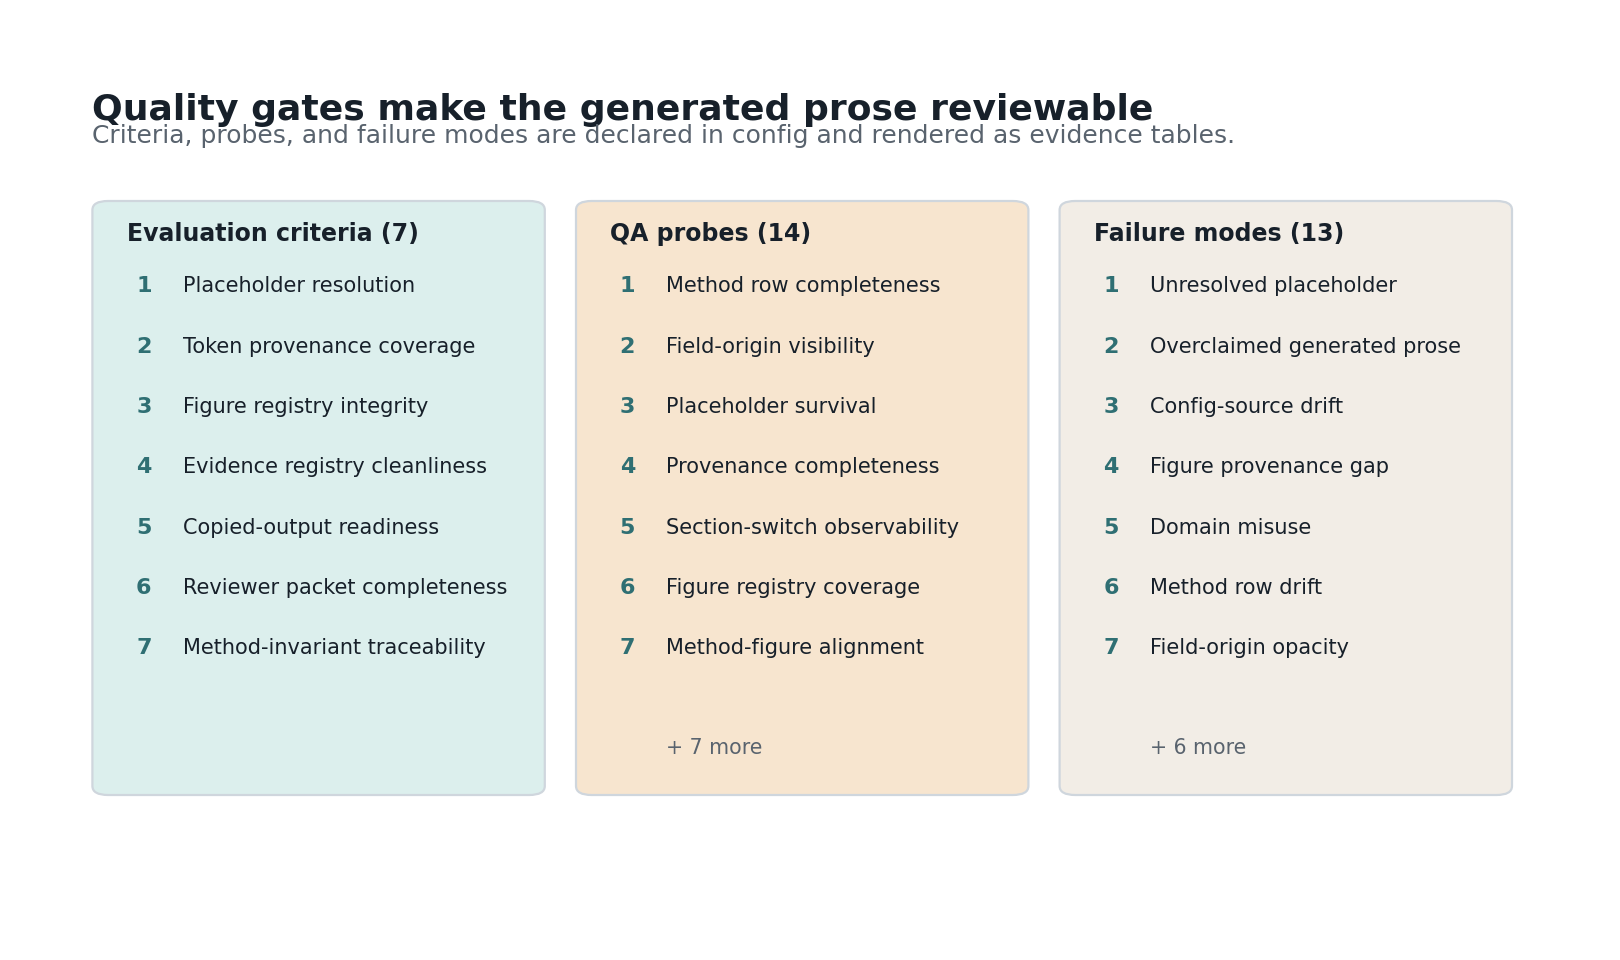
\includegraphics[keepaspectratio,alt={Quality gate matrix}]{../figures/quality_gate_matrix.png}}
\caption{Quality gate matrix}\label{fig:quality-gate-matrix}
\end{figure}
\end{frame}

\begin{frame}[fragile,allowframebreaks]{Evaluation Criteria}
\protect\phantomsection\label{evaluation-criteria}
{\def\LTcaptype{none} % do not increment counter
\begin{longtable}[]{@{}
  >{\raggedright\arraybackslash}p{(\linewidth - 6\tabcolsep) * \real{0.2500}}
  >{\raggedright\arraybackslash}p{(\linewidth - 6\tabcolsep) * \real{0.2500}}
  >{\raggedright\arraybackslash}p{(\linewidth - 6\tabcolsep) * \real{0.2500}}
  >{\raggedright\arraybackslash}p{(\linewidth - 6\tabcolsep) * \real{0.2500}}@{}}
\toprule\noalign{}
\begin{minipage}[b]{\linewidth}\raggedright
Criterion
\end{minipage} & \begin{minipage}[b]{\linewidth}\raggedright
Target
\end{minipage} & \begin{minipage}[b]{\linewidth}\raggedright
Evidence
\end{minipage} & \begin{minipage}[b]{\linewidth}\raggedright
Gate
\end{minipage} \\
\midrule\noalign{}
\endhead
Placeholder resolution & No unresolved uppercase manuscript placeholders
remain in output/manuscript or rendered web output. &
tests/test\_manuscript\_variables.py and rg unresolved-token scan. &
\texttt{pytest} \\
Token provenance coverage & Every selected token maps to category,
selected value, section, and config pointer. &
output/reports/injection\_trace.json and
output/data/token\_inventory.json. & \texttt{analysis} \\
Figure registry integrity & Every referenced figure label is present in
output/figures/figure\_registry.json. & scripts/04\_validate\_output.py
figure registry check. & \texttt{validation} \\
Evidence registry cleanliness & Generated manuscript numbers and claims
pass the project evidence registry. &
output/reports/evidence\_registry.json. & \texttt{validation} \\
Copied-output readiness & PDF, HTML, slides, figures, data, and reports
copy into output/templates/template\_madlib. &
scripts/05\_copy\_outputs.py output statistics. & \texttt{copy} \\
Reviewer packet completeness & Hydrated Markdown, rendered PDF, web
output, slides, figures, data, reports, validation results, and copy
statistics are all present for review. & Stage 04 validation report and
Stage 05 output\_statistics.json. & \texttt{copy} \\
Method-invariant traceability & Token choices can be explained only by
seed, slot, category, ordinal, and ordered category inventory. &
tests/test\_tokens.py and generated Methods digest prose. &
\texttt{pytest} \\
\bottomrule\noalign{}
\end{longtable}
}
\end{frame}

\begin{frame}[fragile,allowframebreaks]{Quality Probes}
\protect\phantomsection\label{quality-probes}
{\def\LTcaptype{none} % do not increment counter
\begin{longtable}[]{@{}
  >{\raggedright\arraybackslash}p{(\linewidth - 6\tabcolsep) * \real{0.2500}}
  >{\raggedright\arraybackslash}p{(\linewidth - 6\tabcolsep) * \real{0.2500}}
  >{\raggedright\arraybackslash}p{(\linewidth - 6\tabcolsep) * \real{0.2500}}
  >{\raggedright\arraybackslash}p{(\linewidth - 6\tabcolsep) * \real{0.2500}}@{}}
\toprule\noalign{}
\begin{minipage}[b]{\linewidth}\raggedright
Probe
\end{minipage} & \begin{minipage}[b]{\linewidth}\raggedright
Question
\end{minipage} & \begin{minipage}[b]{\linewidth}\raggedright
Passing signal
\end{minipage} & \begin{minipage}[b]{\linewidth}\raggedright
Artifact
\end{minipage} \\
\midrule\noalign{}
\endhead
Method row completeness & Does the protocol table cover schema intake,
token planning, composition, figures, validation, copy, and review
handoff? & method\_protocol includes rows for every major pipeline
responsibility. &
\breaktt{manuscript/config.yaml\ and\ output/data/section\_plan.json} \\
Field-origin visibility & Can a reviewer tell which visible fields were
authored and which were defaulted? & Configured-field inventory and
summary tables report explicit and defaulted paths. &
\breaktt{output/data/configured\_field\_inventory.json} \\
Placeholder survival & Did any source token survive hydration? & No
uppercase placeholders are found in generated manuscript or web files. &
\breaktt{output/manuscript\ and\ output/web} \\
Provenance completeness & Can every selected token be traced to a
category, section, value, and config key? & The injection trace and
token inventory contain one row for each generated token. &
\breaktt{output/reports/injection\_trace.json} \\
Section-switch observability & Does a disabled section resolve to a
visible explanation? & Disabled section bodies cite their controlling
section condition. & \breaktt{output/data/section\_plan.json} \\
Figure registry coverage & Does every manuscript figure reference have a
generated registry entry? & Figure registry validation passes. &
\breaktt{output/figures/figure\_registry.json} \\
Method-figure alignment & Do method figures describe generated data
rather than decorative or unsupported claims? & Figure registry
captions, nonblank PNG tests, and manual visual QA align with artifact
data. & \texttt{output/figures} \\
Evidence cleanliness & Do generated claims stay within local evidence
boundaries? & Evidence registry validation passes without unsupported
claims. & \breaktt{output/reports/evidence\_registry.json} \\
Fork readiness & Does the authoring contract tell downstream forks what
to extend before adding domain claims? & Authoring obligations cite
config diffs, claim ledger updates, validators, and full reruns. &
\breaktt{output/manuscript/10\_authoring\_contract.md} \\
Copied-output parity & Did copied deliverables preserve the validated
project output surface? & Copy-stage statistics include PDF, HTML,
slides, figures, data, and reports. &
\breaktt{output/templates/template\_madlib} \\
Digest invariant review & Are the allowed token-selection inputs
documented and protected by tests? & Methods prose names the digest
inputs and token tests prove seed/category sensitivity. &
\breaktt{src/tokens.py\ and\ output/manuscript/02\_methodology.md} \\
Claim-ledger alignment & Do method and documentation claims point to
config, source, generated artifacts, or explicit non-claim boundaries? &
Claim-ledger rows cover expanded method protocol and fork-validator
boundaries. & \breaktt{data/claim\_ledger.yaml} \\
Review packet completeness & Can a reviewer inspect every output surface
needed to audit the method? & Copied outputs include manuscript, web,
slides, figures, data, reports, validation, and copy statistics. &
\breaktt{output/templates/template\_madlib\ and\ output/reports/output\_statistics.json} \\
Fork migration sufficiency & Does the documentation tell forks which
surfaces to change before adding domain claims? & README, STANDALONE,
manuscript README, and Authoring Contract list config, source, test,
validator, and claim-ledger obligations. &
\breaktt{README.md,\ STANDALONE.md,\ manuscript/README.md,\ and\ output/manuscript/10\_authoring\_contract.md} \\
\bottomrule\noalign{}
\end{longtable}
}
\end{frame}

\end{document}
